\documentclass{article}
\usepackage[paperwidth=160mm,paperheight=154mm,margin=0pt]{geometry}
\usepackage[UTF8,fontset=none]{ctex}
\IfFontExistsTF{Microsoft YaHei}{%
  \setCJKmainfont{Microsoft YaHei}
  \setCJKsansfont{Microsoft YaHei}
}{%
  \setCJKmainfont{Noto Sans CJK SC}
  \setCJKsansfont{Noto Sans CJK SC}
}
\usepackage{tikz}
\usepackage{graphicx}
\usetikzlibrary{arrows.meta,positioning,calc}
\begin{document}
\pagestyle{empty}\noindent
\begin{tikzpicture}[x=1mm,y=1mm, every node/.style={font=\sffamily}]
\definecolor{ink}{HTML}{272727}
\definecolor{cyan}{HTML}{E0F0F0}
\definecolor{pink}{HTML}{E4CCD8}
\definecolor{green}{HTML}{F0E0D0}
\definecolor{cream}{HTML}{E0E0F0}
\definecolor{blue}{HTML}{0F4D92}
\definecolor{accentred}{HTML}{B64342}
\fill[white] (0,0) rectangle (160,154);
\fill[cyan] (0,113) rectangle (160,154);
\fill[pink] (0,71) rectangle (160,110);
\fill[green] (0,0) rectangle (160,68);
\node[anchor=west,text=ink,font=\sffamily\bfseries\fontsize{12}{14}\selectfont] at (5,148) {问题一  独立Task的切图与多核调度};
\node[anchor=west,text=ink,font=\sffamily\bfseries\fontsize{10}{12}\selectfont] at (5,137) {01 对象与机理};
\node[anchor=west,text=ink,font=\sffamily\fontsize{9}{11}\selectfont] at (6,125) {二部计算图 $G=(\mathcal O\cup\mathcal T,E)$};

\foreach \x/\y/\label/\col in {82/128/$o_1$/pink,103/134/$t_1$/cream,103/122/$t_2$/cream,126/128/$o_2$/pink,145/128/$t_3$/cream}{\node[circle,draw=blue!65,fill=\col,minimum size=8mm,font=\fontsize{8}{9}\selectfont] at (\x,\y) {\label};}
\draw[blue,thick,-{Latex[length=2mm]}] (86,130)--(99,133);
\draw[blue,thick,-{Latex[length=2mm]}] (86,126)--(99,123);
\draw[blue,thick,-{Latex[length=2mm]}] (107,133)--(122,130);
\draw[blue,thick,-{Latex[length=2mm]}] (107,123)--(122,126);
\draw[blue,thick,-{Latex[length=2mm]}] (130,128)--(140,128);
\node[text=ink,font=\fontsize{7.5}{9}\selectfont] at (114,116) {操作—张量交替；箭头为依赖};

\node[anchor=west,text=ink,font=\sffamily\bfseries\fontsize{10}{12}\selectfont] at (5,103) {02 方法与约束};
\node[rounded corners=1mm,draw=blue!50,fill=white,minimum width=43mm,minimum height=19mm,align=center,text=ink,font=\sffamily\fontsize{8.6}{10.5}\selectfont] (a) at (26,89) {非COPY操作\\弱连通块};
\node[rounded corners=1mm,draw=blue!50,fill=white,minimum width=43mm,minimum height=19mm,align=center,text=ink,font=\sffamily\fontsize{8.6}{10.5}\selectfont] (b) at (80,89) {连通块分核\\深度分段／宽图分批};
\node[rounded corners=1mm,draw=blue!50,fill=white,minimum width=43mm,minimum height=19mm,align=center,text=ink,font=\sffamily\fontsize{8.6}{10.5}\selectfont] (c) at (134,89) {每子图一个Task\\边界张量经DDR};
\draw[blue,thick,-{Latex[length=2mm]}] (a.east) -- (b.west);
\draw[blue,thick,-{Latex[length=2mm]}] (b.east) -- (c.west);
\node[anchor=west,text=ink,font=\sffamily\fontsize{8.2}{10}\selectfont] at (5,74) {$S_k=T_1/T_k$；最小化官方全局完成周期 $T_k$};
\node[anchor=west,text=ink,font=\sffamily\bfseries\fontsize{10}{12}\selectfont] at (5,62) {03 实测结果与核验};
\node[anchor=west,text=ink,font=\sffamily\bfseries\fontsize{8.8}{10.5}\selectfont] at (5,52) {100例五核平均加速比 $3.5093$；中位数 $4.1473$};
\node[anchor=west,text=ink,font=\sffamily\fontsize{8.3}{10}\selectfont] at (5,44) {500个所选配置通过官方评估与独立时间线核验};
\node[anchor=west] at (5,21) {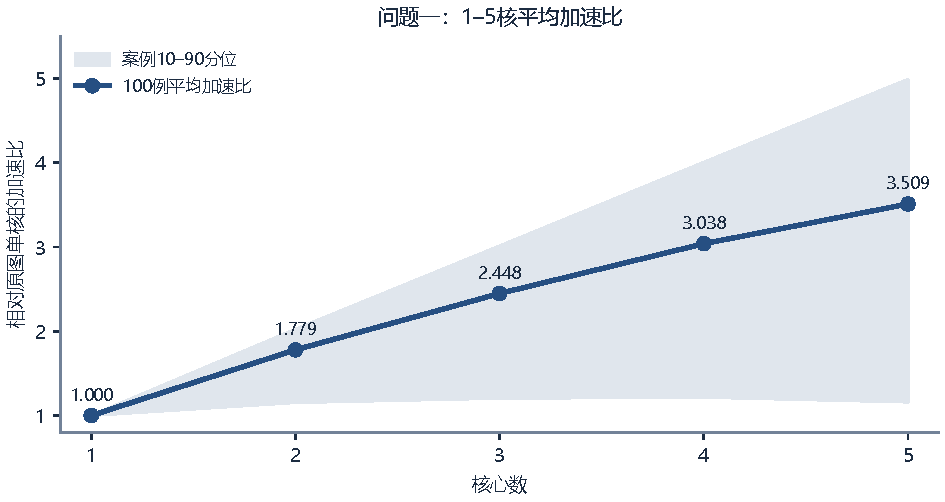
\includegraphics[width=72mm,height=30mm,keepaspectratio]{../正式图件/q1-F02.pdf}};
\node[anchor=east] at (155,21) {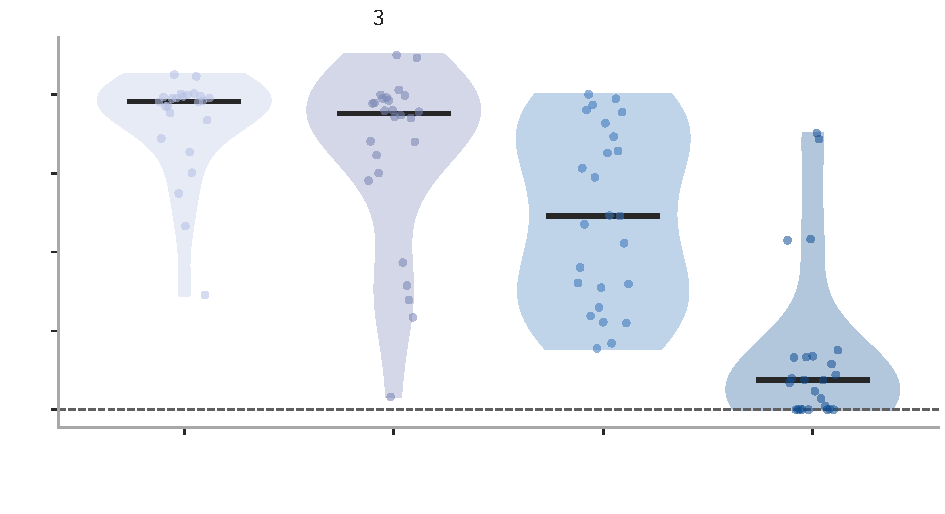
\includegraphics[width=72mm,height=30mm,keepaspectratio]{../正式图件/q1-F03.pdf}};
\node[anchor=west,text=ink,font=\sffamily\fontsize{7.5}{9}\selectfont] at (5,4) {细节参见正文图 q1-F02、q1-F03；缩图仅作证据导航。};
\end{tikzpicture}
\end{document}
